%
% RoboCert Graphical notation (using TikZ)
%
% Last updated: 2022-08-26
%

\newcommand{\rckeywordfont}{\sffamily\bfseries}
\newcommand{\rckeyword}[1]{{\rckeywordfont #1}}
\newcommand{\rcosigil}{\rckeyword{op}}
\newcommand{\rcesigil}{\rckeyword{event}}

\newlength{\rctopmargin}
\setlength{\rctopmargin}{3em}

\newlength{\rcstepmargin}
\setlength{\rcstepmargin}{.2em}

% Shading used for various parts of the graphical notation.
% Colour to be used very sparingly here.
\colorlet{rcshading}{black!20}

\usetikzlibrary{arrows.meta,matrix,shapes,calc,fit}
\tikzset{
    rcseq/.style={row sep=2.2em, column sep=8em},
% Actors
    rcactor/.style={draw, rectangle, minimum width=4em, align=center, minimum height=1.7em, fill={rcshading}, font={\footnotesize\sffamily}},
% Control flow
    rclifeline/.style={thick},
    cfbox/.style={draw, solid},
    cfheader/.style={chamfered rectangle, draw, font={\scriptsize\sffamily}, fill={rcshading}, chamfered rectangle corners=south east, inner sep=0.1em},
    branchdiv/.style={draw, thick, dotted},
    guard/.style={font={\scriptsize\sffamily}, anchor=north east, align=right, inner sep=0.2em},
% Deadlines
    deadline/.style={solid, font={\scriptsize}},
    deadlinespan/.style={latex-latex},
% Temperature modalities
    cold/.style={thick, solid},
    hot/.style={cold, double},
% Occurrences
    arrow/.style={->, cold},
    arrowlabel/.style={fill=white, font={\scriptsize\sffamily}, inner sep=0.2em},
    wait/.style={cold, font={\scriptsize}},
    end/.style={fill, very thick, rectangle, minimum height=3pt, minimum width=15pt, inner sep=0em}
}

% pseudo-UML stereotype name
% #1: name of the stereotype
\newcommand{\rcstereotype}[1]{\rckeyword{\(\langle\!\langle\)\,#1\,\(\rangle\!\rangle\)}}

% Target actor
\newcommand{\rctarget}{\rcstereotype{target}}

% Component actor
% #1: name of the type
\newcommand{\rccomponent}[1]{\rcstereotype{component} #1}

\newcommand{\gdiff}[2]{#1\setminus#2}
\newcommand{\guniverse}{\ast}
\newcommand{\gextset}[1]{\{#1\}}
\newcommand{\gemptyset}{\gextset{}}
\newcommand{\grefset}[1]{\textsf{#1}}

% Header for sequence diagrams
%
% #1: name of diagram
% #2: name of target
\newcommand{\rcseq}[2]{\rckeyword{sd} #1 (#2)}

% Combined fragment or diagram frame
% #1: padding factor
% #2: top-left
% #3: bottom-right
% #4: header
\newcommand{\rcframe}[4]{
  % Slightly eccentric definition here to line the world up with the RHS,
  % and leave room for the top 'sd' line.
  \draw ($(#2) + (-#1*\the\rcstepmargin, \the\rctopmargin)$) rectangle ($(#3) + (#1*\the\rcstepmargin, -#1*\the\rcstepmargin)$);
  \node[cfheader, anchor=north west] at ($(#2) + (-#1*\the\rcstepmargin, \the\rctopmargin)$) {\footnotesize #4};
}

% Guard
% #1: name
% #2: position (right edge of box)
% #3: expression
\NewDocumentCommand{\gguard}{m m m}{\node[guard] (#1) at (#2) {[#3]};}

% Wildcard with an optional binding
\NewDocumentCommand{\gwildcard}{o}{\rckeyword{any}\IfValueT{#1}{ \rckeyword{as} #1}}
\NewDocumentCommand{\gusebinding}{m}{\rckeyword{@}#1}

% The 'otherwise' guard
\NewDocumentCommand{\gotherwise}{}{otherwise}

% Loop
% #1: coordinates to fit
% #2: loop name
% #3: loop header
% (#4: inner sep)
% (#5: horizontal inner sep)
\NewDocumentCommand{\gloop}{m m m O{0.4em} O{0}}{\gcfrag{#1}{#4}{\rckeyword{loop}#3 #2}{loop#2}[cfbox][#5]}

% Gap
% #1: top-left
% #2: name
% #3: set
% (#4: inner sep)
% (#5: horizontal inner sep)
\NewDocumentCommand{\guntil}{m m m O{0.3em} O{1.1em}}{\gcfrag{#1}{#4}{\rckeyword{any}(\(#3\)) \rckeyword{until} }{#2}[cfbox][#5]}

% Branch division
% #1: name of branch
% #2: right
\NewDocumentCommand{\gbranchdiv}{m m}{
  \draw (#2 -| brbranch#1)
        edge[branchdiv]
        (#2 -| branch#1.west)
  ;
}

% Branch
% #1: fit
% #2: branch name
% #3: branch header
\NewDocumentCommand{\gbranch}{m m m}{\gcfrag{#1}{0.1em}{#3 #2}{branch#2}}

% Alternative branch header
\NewDocumentCommand{\galternative}{}{\rckeyword{alt}}
% X-Alternative branch header
\NewDocumentCommand{\gxalternative}{}{\rckeyword{xalt}}
% Parallel branch header
\NewDocumentCommand{\gparallel}{}{\rckeyword{par}}
% Optional block header
\NewDocumentCommand{\gopt}{}{\rckeyword{opt}}


% Loop bounds
% These follow UML for now.
\newcommand{\gloopinfinite}{}
\newcommand{\gloopdefinite}[1]{(#1)}
\newcommand{\glooprange}[2]{(#1, #2)}
\newcommand{\glooplower}[1]{\glooprange{#1}{\(\ast\)}}

% Generic message command
% #1: LHS
% #2: RHS
% #3: sigil
% #4: label
% #5: temperature
\NewDocumentCommand{\gmessage}{m m m m m}{\draw (#1) edge[arrow, \IfBooleanTF{#5}{hot}{cold}] node[arrowlabel] {#3\(\;\)#4} (#2);}

% #1: temperature (star)
% #2: LHS
% #3: RHS
% #4: label
% #5: argument(s)
\NewDocumentCommand{\goperation}{s m m m m}{\gmessage{#2}{#3}{\osigil}{#4(#5)}{#1}}

% #1: temperature (star)
% #2: LHS
% #3: RHS
% #4: label
% #5: return value (optional)
\NewDocumentCommand{\gevent}{s m m m o}{\gmessage{#2}{#3}{\esigil}{#4\IfValueT{#5}{(#5)}}{#1}}

% #1: temperature (star)
% #2: LHS
% #3: RHS
% #4: units expression
\NewDocumentCommand{\gwait}{s m m m}{\draw (#2) edge[wait, \IfBooleanTF{#1}{hot}{cold}] node[arrowlabel] {\rckeyword{wait}(#4)} (#3);}

\newcommand{\gdeadlinehoffset}{0.6em}
\newcommand{\gdeadlinevoffset}{0.5em}
% #1: Top
% #2: Bottom
% #3: Bounds set
% #4: Lower bound
\NewDocumentCommand{\gdeadline}{m m m}{
  \draw[deadline]
    ($(#1) + (0, \gdeadlinevoffset)$)
      --
    ($(#1) + (-\gdeadlinehoffset, \gdeadlinevoffset)$);
  \draw
    ($(#2) + (-\gdeadlinehoffset, -\gdeadlinevoffset)$)
      edge[deadlinespan] node[font=\scriptsize, anchor=east, inner sep=0.2em] {#3}
    ($(#1) + (-\gdeadlinehoffset, \gdeadlinevoffset)$)
      edge[deadline]
    ($(#2) + (0, -\gdeadlinevoffset)$);
}

We define \langname{} by defining its
metamodel.  Parts of the metamodel map to various concrete notations (for
instance, sequences map to UML-style sequence diagrams), and have a semantics
in terms of process algebras and other formalisms (\cref{cha:semantics-intro}).

This chapter discusses the top-level metamodel and, in turn, the key concepts
of \langname.

\section{Introduction}\label{ssec:core-metamodel-intro}
\subsection{How to read the rest of this chapter}\label{ssec:core-metamodel-intro-readme}

Each section, except this one,
introduces a group of top-level \langname{}
functionality in a top-down manner.  These sections contain:

\begin{itemize}
\item
	a class diagram representing the Ecore classes, enumerations, and other
	components that make up the group being discussed;
\item
	descriptions of the components being shown in the class diagram;
\item
	where relevant, examples of the components in terms of the concrete
	syntaxes of \langname.
\end{itemize}

\section{Top-level}\label{sec:core-metamodel-top}
% !TEX root=../../robocert.tex
\begin{figure}[htb]
  \centering
  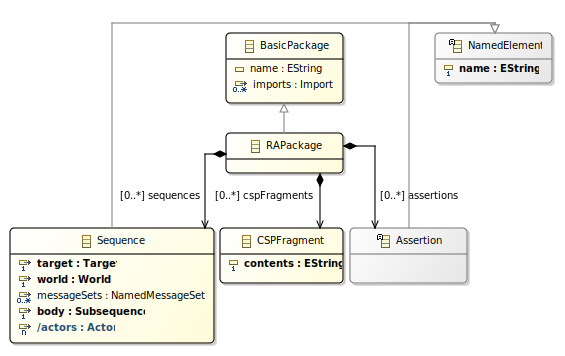
\includegraphics[width=.85\textwidth]{diagrams/Top}
  \caption{Class diagram for the top of the \langname{} metamodel.}
  \label{fig:metamodel-top}
\end{figure}

\Cref{fig:metamodel-top} is the top-level metamodel diagram for \langname.

Each \langname{} script contains an \mrapackage,\footnote{\mrapackage{} stands
  for `RoboStar Assertions package'; we use this name because \mrcpackage{} is
  already used for RoboChart packages.}
which is a type of RoboStar \mbasicpackage.
Each \mrapackage{} can contain zero or more of each of these types of content:

\begin{itemize}
\item
  \msequencegroup:
  a sequence diagram group
  (see \cref{sec:metamodel-sequences});
\item
  \mcspfragment:
  a CSP fragment, currently not bound to a particular process
  \todo{this will change};
\item
  \massertion:
  an assertion
  (see \cref{sec:core-metamodel-assertions}).
\end{itemize}

%%% Local Variables:
%%% mode: latex
%%% TeX-master: "../../robocert"
%%% End:


\section{Assertions}\label{sec:core-metamodel-assertions}
%!TEX root=../robocert.tex
\begin{figure}
	\centering
	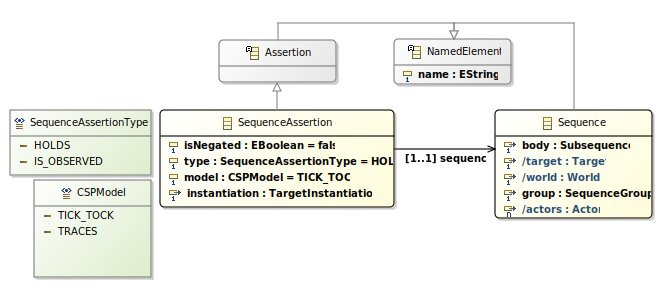
\includegraphics[width=0.7\textwidth]{diagrams/Assertions}
	\caption{Class diagram for the part of the \langname{} metamodel dealing with assertions.}
	\label{fig:metamodel-assertions}
\end{figure}

\Cref{fig:metamodel-assertions} depicts the part of the metamodel concerning
assertions.

\subsection{\massertion}

An \massertion{} is an named assertion statement.  Currently, there is
only one type of assertion: a \msequenceassertion{}.  \todo{This will change
when merging with the existing language, if not sooner.}

\subsection{\msequenceassertion}\label{ssec:metamodel-assertions-sequence}

A \msequenceassertion{} is an assertion about a particular \msequence{} with
respect to its \mtarget.  The \mtarget{} is modified by applying an
assertion-level \mtargetinstantiation, which may fix any constants not bound
by the sequence-level instantiation.  (The default is an empty instantiation,
meaning the target is exactly as specified at the sequence level.)

The specific sequence assertion type comes from the \msequenceassertiontype:
either `sequence holds on target' (refinement), or `sequence is observed on
target' (reverse refinement).  The assertion can be negated.  The choice of
\mcspmodel{} affects how the assertion is checked with CSP tools such as FDR
\todo{the models aren't actually used yet; everything is treated as untimed
traces refinement.  This will change.}

\begin{lstlisting}[style=Example]
assertion A: SequenceName holds           // positive 'holds' SequenceAssertion
assertion B: SequenceName does not hold   // negative 'holds' SequenceAssertion
assertion C: SequenceName is observed     // positive 'is observed' SequenceAssertion
assertion D: SequenceName is not observed // negative 'is observed' SequenceAssertion

assertion E: SequenceName holds with { CONSTANT set to 5 }
// example of SequenceAssertion with custom TargetInstantiation
\end{lstlisting}

%%% Local Variables:
%%% mode: latex
%%% TeX-master: "../robocert"
%%% End:


%%% Local Variables:
%%% mode: latex
%%% TeX-master: "../robocert"
%%% End:
